\documentclass{article}

\usepackage[utf8]{inputenc}
\usepackage[letterpaper,top=1.5cm,bottom=1.5cm,left=2cm,right=2cm,marginparwidth=1.75cm]{geometry}
\usepackage[english]{babel}
\usepackage[skip=2pt]{caption}
\usepackage{graphicx}
\usepackage[colorlinks=false, allcolors=black, hidelinks=true]{hyperref}
\usepackage{biblatex}
\usepackage{makecell}
\usepackage{appendix}
\usepackage{amsmath}

\addbibresource{IVI.bib}

\title{Interactive Visualizations (IVI) Bericht}
\author{Nicola Rohner}
\date{SE FE 2023}

\begin{document}

\maketitle

\begin{center}
\textbf{Repository:} \url{https://github.com/nicolarohner1337/ivi}
\end{center}

\begin{abstract}
In diesem Bericht werden die Lernergebnisse des Moduls IVI zusammengefasst.\\
Für alle ausser LE1 wurden folgende Daten verwendet: \newline
GroupLens Research hat Bewertungsdatensätze von der MovieLens-Website \url{https://movielens.org} gesammelt und zur Verfügung gestellt.
Die Datensätze wurden über verschiedene Zeiträume hinweg gesammelt, abhängig von der Grösse des Satzes. Das ZIP findet man unter folgendem Link: \url{https://files.grouplens.org/datasets/movielens/ml-latest.zip}
Die Daten umfassen 27.000.000 Bewertungen und 1.100.000 Tag-Anwendungen für 58.000 Filme von 280.000 Nutzern. Beinhaltet Tag-Genom-Daten mit 14 Millionen Relevanz-Scores für 1.100 Tags.\\
\noindent\\
Die Visualisierungen in diesem Bericht wurden alle selbst erstellt. 
Der Datensatz wurde bereits für die Challenge CDS1 genutzt und für die Erarbeitung von GDV.
\end{abstract}

\tableofcontents

\newpage

\section{LE1: Performance}
In Zeiten von Big Data ist es wichtig, dass Visualisierungen schnell und performant sind. In diesem LE wird untersucht, wie sich die Performance von Visualisierungen auf verschiedene Arten beeinflussen lässt.


\subsection{WebGL}
WebGL ist eine leistungsstarke Technologie, die Berechnungen beschleunigt. Allerdings gibt es einige Einschränkungen.
WebGL benötigt eine GPU (Grafikkarte), die nicht immer in allen Browsern verfügbar ist.
Die CPU verarbeitet alle Hauptfunktionen des Computers, während die GPU viele kleinere Aufgaben gleichzeitig ausführt.\cite{noauthor_cpu_nodate}

%make 5x2 table
%how can i align the text in the cells?
\begin{table}[!h]
\centering
\begin{tabular}{|l|l|}
\hline
\textbf{CPU} & \textbf{GPU} \\
\hline
\makecell[l]{Generalistische Komponente - Verarbeitet die \\ wichtigsten Verarbeitungsfunktionen eines Computers}& \makecell[l]{Spezialisierte Komponente - Verarbeitet \\Grafik- und Video-Rendering} \\
\hline
Kernanzahl- 2-64 (die meisten CPUs)&Kernanzahl- Tausende \\
\hline
Führt Prozesse seriell aus & Führt Prozesse parallel aus\\
\hline
\makecell[l]{Besser bei der Verarbeitung\\ einer grossen Aufgabe zur gleichen Zeit} & \makecell[l]{Besser bei der Verarbeitung \\mehrerer kleinerer Aufgaben zur gleichen Zeit} \\
\hline
\end{tabular}
\caption{\label{tab: LE1 CPU vs GPU}CPU vs GPU}
\end{table}
    
\noindent
Mit WebGL gerenderte Daten werden als Pixelraster gezeichnet, was in einigen Fällen zu verpixelten oder unscharfen Bildern führen kann.
Browser begrenzen die Anzahl der WebGL Kontexte, auf die ein bestimmtes Webdokument zugreifen kann, was die Darstellung von WebGL-Visualisierungen einschränken kann.
Browser setzen Grenzen für die Höhe und Breite von Visualisierungen, die WebGL verwenden, was bei extrem grossen Plots zu Problemen führen kann.\cite{plotly_webgl_nodate}
%hard break
\newline
\newline
Um die Performance Unterschiede zu untersuchen habe ich eine Visualisierung erstellt, welche 100000 zufällige Punkte in einem 2D Koordinatensystem darstellt.
Einmal wurde die Visualisierung mit dem Modus SVG und einmal mit WebGL gerendert. Was bereits qualitativ auffällt ist, dass die WebGL Visualisierung deutlich schneller angezeigt wird im Chrome Browser.

%enter image here
\begin{figure}[!h]
\centering
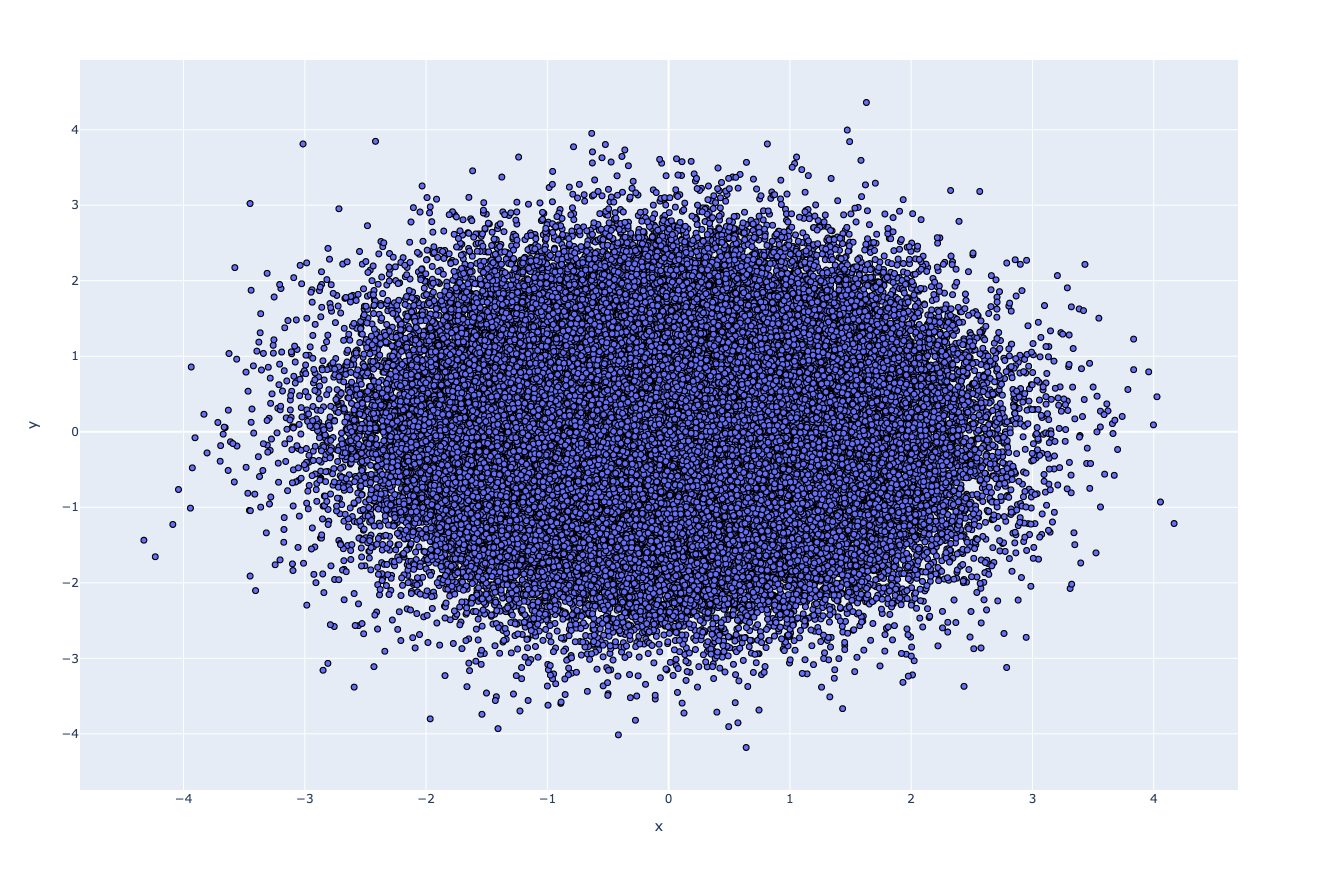
\includegraphics[width=0.2\textwidth]{img/random_dots.png}
\caption{\label{fig: LE1 Random Dots plot}Random dots}
\end{figure}

\noindent
Die Chrome Entwickler Tools verfügen über ein Performance Profiler Tool, welches die Performance einer Webseite analysieren kann. Es unterteilt die Laufzeitleistung in das RAIL-Modell\cite{noauthor_measure_nodate}: Response, Animation, Idle und Load.
Im Kontext zur Visualisierung betrachte man die Scripting, Rendering und Painting Kategorien.\cite{kayce_basques_analyze_nodate}

%enter table here
\begin{table}[!h]
\centering
\begin{tabular}{|l|l|l|l|}
\hline
\textbf{Kategorie} & \textbf{SVG} & \textbf{WebGL} & \textbf{\%$\Delta$} \\
\hline
Scripting & 3778ms & 651ms & -580\% \\
\hline
Rendering & 2026ms & 14ms & -1447\% \\
\hline
Painting & 197ms & 2ms & -985\% \\
\hline
\end{tabular}
\caption{\label{tab: LE1 Performance}Performance Unterschiede}
\end{table}

\noindent
Zu beobachten ist ein signifikanter Unterschied in den Rendering und Painting Zeiten der beiden Visualisietungen. Auch die subjektive Wahrnehmung der Performance ist deutlich besser bei der WebGL Visualisierung.
Auch die Tradeoffs zwischen Performance und Qualität sind deutlich zu erkennen. Die SVG Visualisierung ist deutlich schärfer und die Punkte sind deutlich besser zu erkennen.
\begin{figure}[!h]
\centering
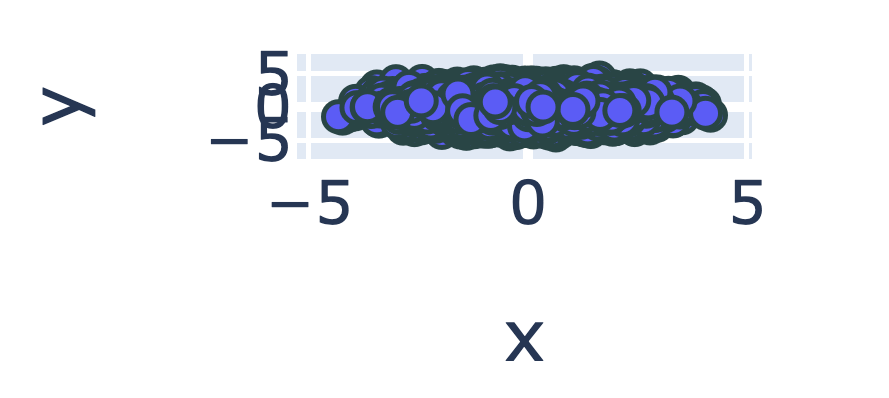
\includegraphics[width=0.2\textwidth]{img/svg_quality.png}
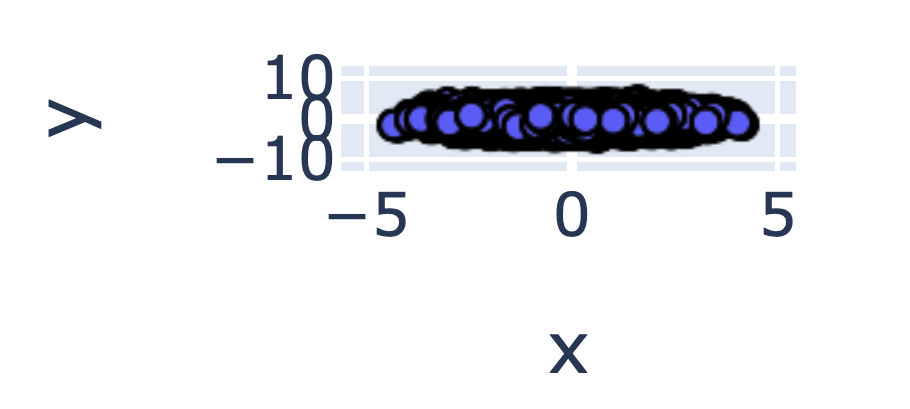
\includegraphics[width=0.2\textwidth]{img/webgl_quality.png}
\setlength{\belowcaptionskip}{-10pt}
\caption{\label{fig: LE1 Qualität Unterschiede} Qualität Unterschiede links SVG, rechts WebGL}
\end{figure}
\newpage

\subsection{Tiling}

Tiling kann die Performance von interaktiven Visualisierungen von grossen Datenmengen verbessern, 
indem es die Daten in kleinere Kacheln aufteilt und nur die benötigten Teile lädt und darstellt. 
Dadurch wird die Rechenleistung effektiver genutzt und die Belastung auf den Computer verringert. 
Die interaktive Natur von Tiling ermöglicht es den Benutzern, schnell und einfach zwischen verschiedenen 
Ausschnitten der Daten zu navigieren und eine schnellere und reaktionsfähigere Erfahrung zu erleben.\cite{noauthor_map_nodate}
Datashader ist ein Grafik-Pipeline-System zur schnellen und flexiblen Erstellung aussagekräftiger Darstellungen grosser Datensätze. Datashader unterteilt die Erstellung von Bildern in eine Reihe expliziter Schritte, die es ermöglichen, Berechnungen an Zwischendarstellungen vorzunehmen.\cite{wong_abstract_2013}
\\
\\
Wir visualisieren hier die räumliche Verteilung der Taxifahrten in New York City. 
Die Daten werden von Plotly zu Verfügung gestellt und sind unter folgendem Link zu finden: \url{https://raw.githubusercontent.com/plotly/datasets/master/uber-rides-data1.csv}

\begin{table}[!h]
\centering
\begin{tabular}{|l|l|}
\hline
\textbf{Date/Time} & \textbf{The date and time of the Uber pickup} \\
\hline
\textbf{Lat} & \textbf{The latitude of the Uber pickup} \\
\hline
\textbf{Lon} & \textbf{The longitude of the Uber pickup} \\
\hline
\end{tabular}
\caption{\label{tab: LE1 Newyork Taxi Data} Newyork Uber Data}
\end{table}



%enter image here
\begin{figure}[!h]
\centering
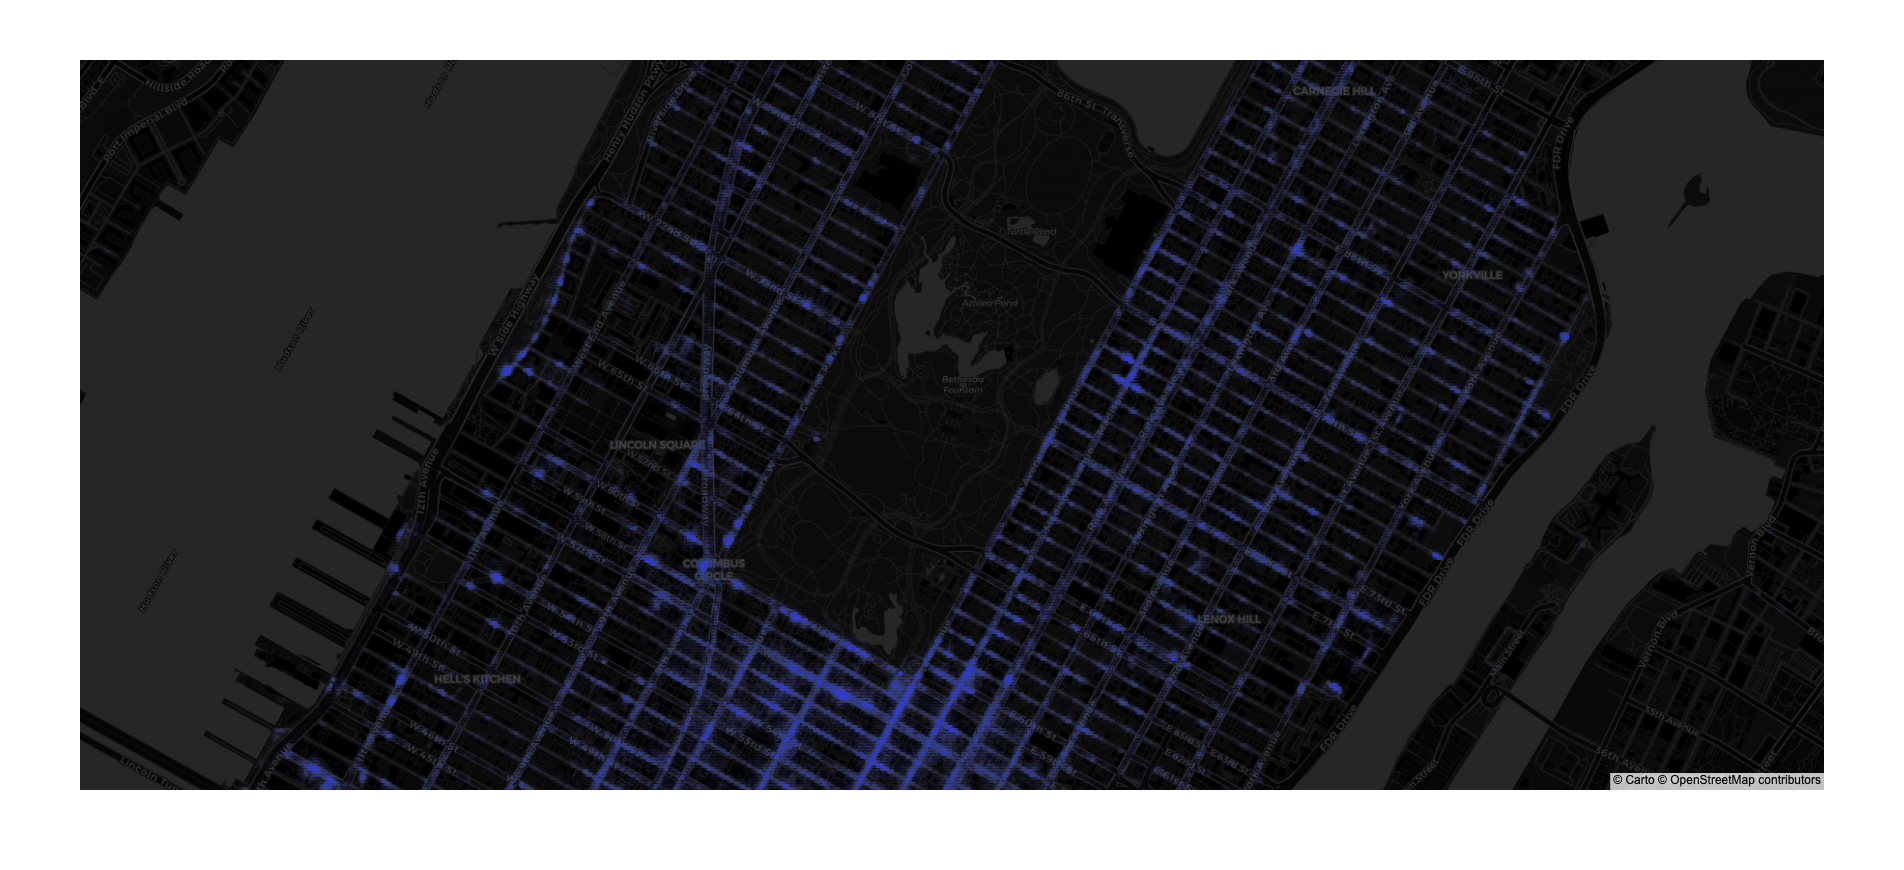
\includegraphics[width=0.4\textwidth]{img/newyork_plotly.png}
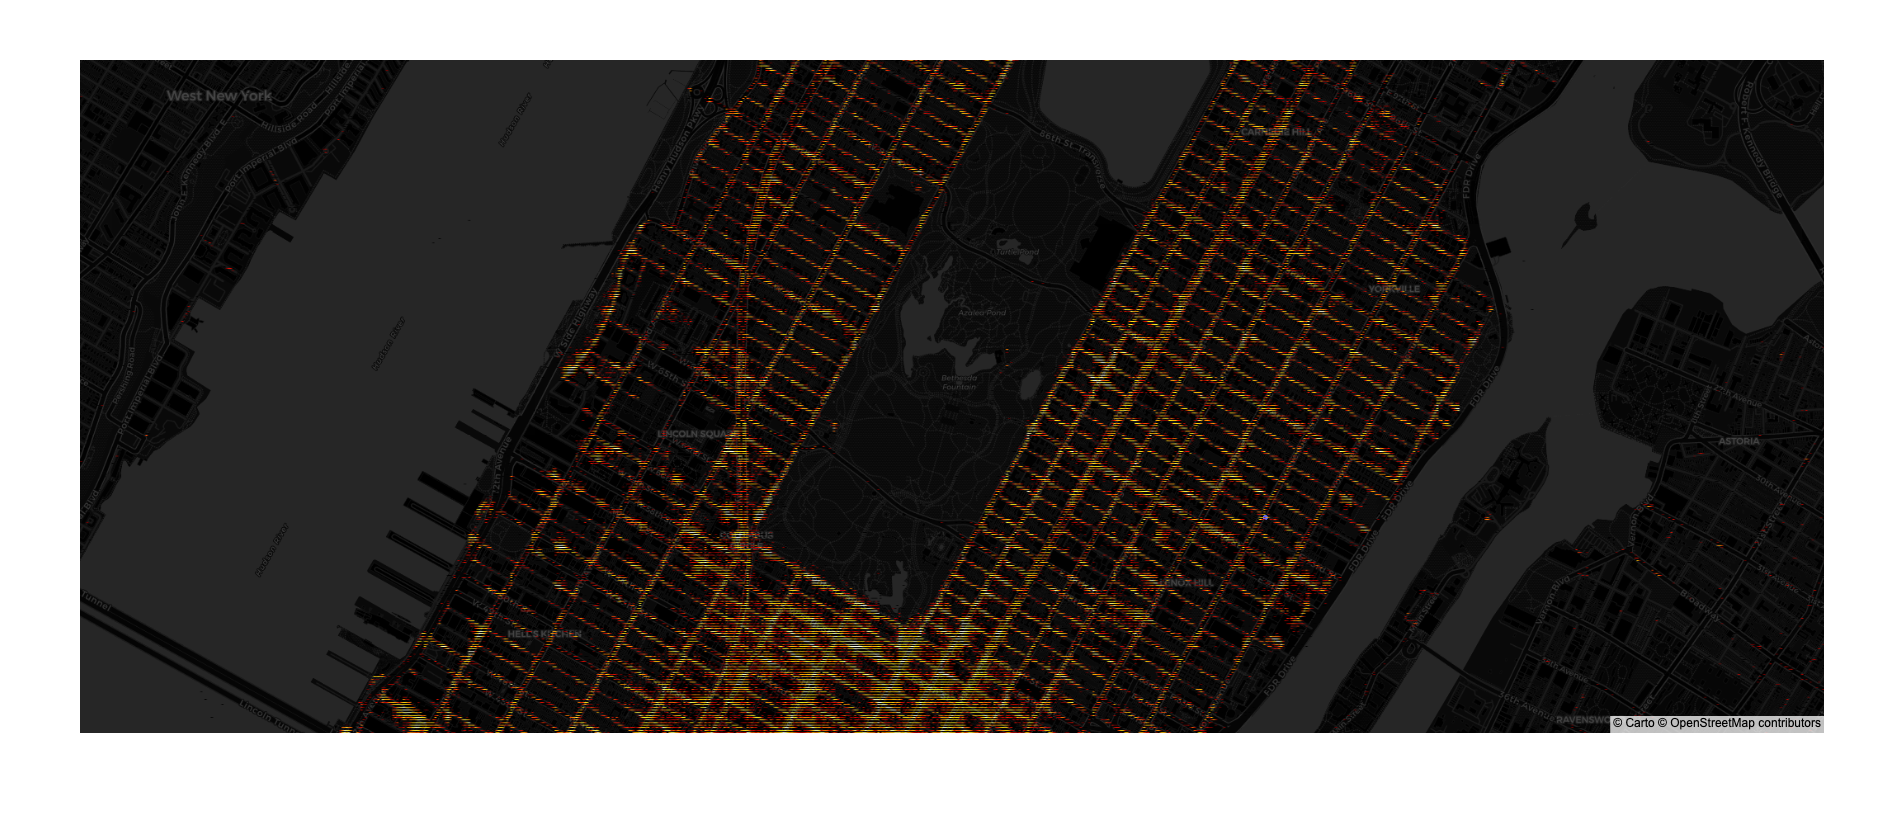
\includegraphics[height=0.18\textwidth]{img/newyork_datashader.png}
\caption{\label{fig: LE1 Plotly vs Datashader} Taxifahrten in Newyork (Plotly links, Datashader Tiles rechts)}
\end{figure}
\noindent
Zu beobachten ist das die unprozessierten Daten mit Plotly zwar schöner dargestellt werden. Aber viel länger brauchen um angezeigt zu werden. Die Datashader Visualisierung ist deutlich schneller und die Daten werden deutlich besser dargestellt.
Diese Beobachtungen wiederspiegeln sich auch in den Performance Daten. Zwar wird nur die Scripting Zeit signifikant verkürzt.


%enter table here
\begin{table}[!h]
    \centering
    \begin{tabular}{|l|l|l|l|}
    \hline
    \textbf{Kategorie} & \textbf{Plotly} & \textbf{Datashader Tile} & \textbf{\%$\Delta$} \\
    \hline
    Scripting & 1241ms & 492ms & -39\% \\
    \hline
    Rendering & 6ms & 6ms & $\pm$0\% \\
    \hline
    Painting & 12ms & 12ms & $\pm$0\% \\
    \hline
    \end{tabular}
    \caption{\label{tab: LE1 Performance}Performance Unterschiede}
\end{table}
\noindent
Spannender bei diesem Fall sind die Unteschiede des genutzen Speichers. Wenn wir den JavaScript Heap betrachten sehen wir einen signifikanten Unterschied.\cite{noauthor_memory_2023}
Plotly braucht fast 130MB um die Daten zu visualisieren, der Datashader Tile braucht nur 23MB.

%enter image here
\begin{figure}[!h]
\centering
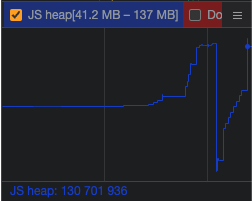
\includegraphics[width=0.2\textwidth]{img/js_heap_plotly.png}
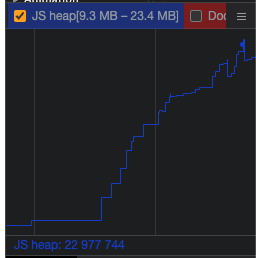
\includegraphics[height=0.158\textwidth]{img/js_heap_datashader.png}
\caption{\label{fig: LE1 Datashader Memory} Memory Heap Plotly vs. Datashader Tile}
\end{figure}
\noindent
Einen ähnlichen Ansatz verfolgen auch Framworks wie Deck.gl. Diese Frameworks sind jedoch auf WebGL basiert und können somit nur auf Browsern mit WebGL Unterstützung verwendet werden.
Sie prozessieren für verschiedene Ansichte voragregierte Tiles und können so sehr schnell und performant visualisieren.\cite{deckgl_home_nodate}

\newpage

\section{LE2: Grundsätze für die Gestaltung von Dashboards}

Ein wichtiger Aspekt bei der Entwicklung von Dashboards ist das Konzept. Dabei hat der Benutzer Zugriff auf verschiedene Steuerelemente und mehrere verknüpfte Visualisierungen. Diese Designprinzipien sind entscheidend für die Entwicklung eines erfolgreichen Dashboards.

\subsection{Schneiderman’s Mantra}
Schneiderman's Mantra ist ein Organisationsprinzip für die Erstellung von Visualisierungssystemen. Es lautet wie folgt:\\ \\
\noindent
\textbf{Overview first}: Im Überblicksschritt wird der gesamte Datensatz in einer geeigneten Anzeigemethode dargestellt. Dies bietet einen Überblick auf hoher Ebene und gibt Kontext für die nächsten Schritte in der Visualisierung.\\ \\
\textbf{Zoom and filter}: Zoomen auf einen Abschnitt des Datensatzes ermöglicht das Entfernen von überflüssigen Daten anhand der angezeigten Koordinaten. So erhalten die relevanten Daten mehr Auflösung und Detail. Das Filtern entfernt überflüssige Daten basierend auf gewünschten Attributen, vereinfacht die Anzeige Ihrer Daten und schafft mehr Platz für Details.\\ \\
\textbf{Details on demand}: Details auf Abruf geben dem Benutzer Kontrolle über die Daten und ermöglichen es, ohne Überladen des Bildschirms weiter zu erkunden. Das Tooltip ist die häufigste Implementierung. Eine andere Möglichkeit besteht darin, ein Feld auszuwählen und die Daten hervorzuheben.\cite{hampdatavisualization_schneidermans_2016}
\\
Eine mögliche Umsetzung mit diesem Prinzip könnte wie folgt aussehen. Im ersten Schritt wird eine Übersicht über die Anzahl Filme pro Genre gegeben.


\begin{figure}[!h]
\centering
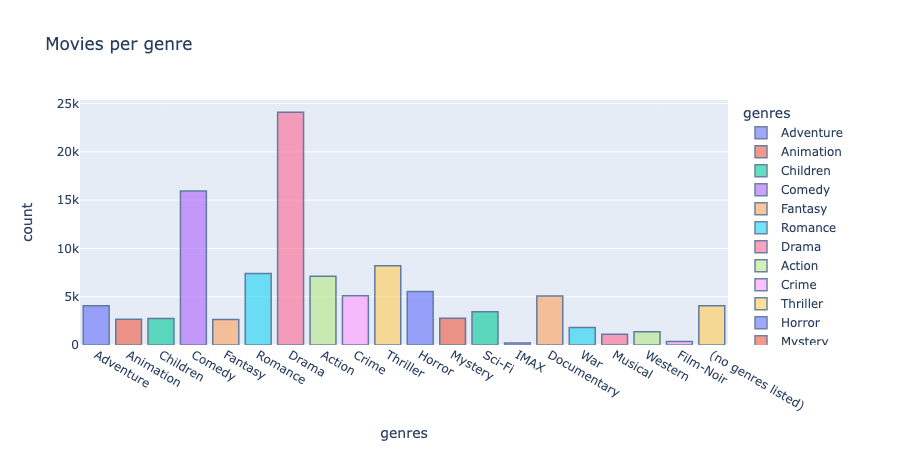
\includegraphics[width=0.4\textwidth]{img/movies_genre.png}
\caption{\label{fig: LE2 Schneiderman Overview} Genre Übersicht}
\end{figure}


Wenn der Benutzer nun auf ein Genre klickt oder auf ein Genre zoomt wird die Anzahl Filme pro Jahr angezeigt.\\

\begin{figure}[!h]
\centering
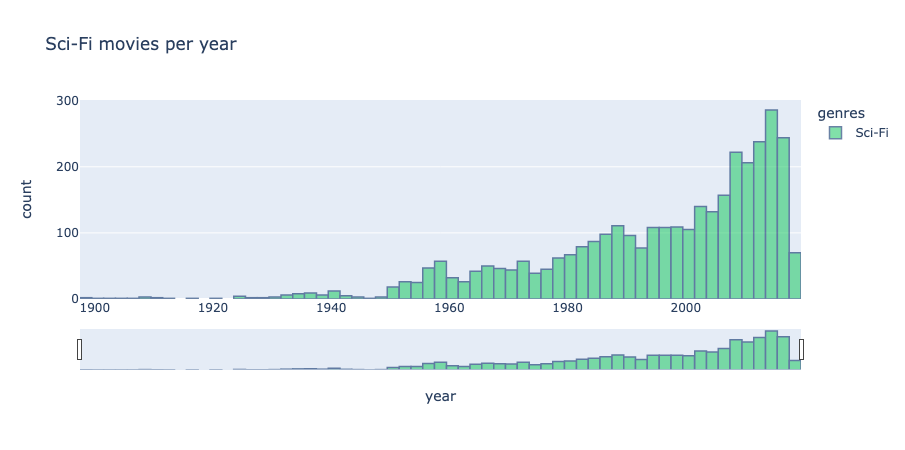
\includegraphics[width=0.4\textwidth]{img/movies-scifi.png}
\caption{\label{fig: LE2 Schneiderman Zoom} Filtering/Zooming: Anzahl Filme pro Jahr}
\end{figure}


Mit einem Tooltip kann der Benutzer nun die Details zum einzelnen Film einsehen.

\begin{figure}[!h]
\centering
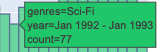
\includegraphics[width=0.2\textwidth]{img/tooltip.png}
\caption{\label{fig: LE2 Schneiderman Zoom} Tooltip: Details on demand}
\end{figure}
Diese Interaktionen können mit Hilfe Plotly.js Chart Events realisiert werden. Wenn ein solches Event getriggert wird kann die Funktion \texttt{Plotly.restyle} aufgerufen werden. Diese Funktion ermöglicht es die Daten eines Charts zu ändern.\\


\newpage
\subsection{Verknüpfte Ansichten}
Das Paradigma der verknüpften Ansichten ist eine Methode, die mehrere einfache Ansichten von Daten verwendet. Wenn Sie mit einer Ansicht interagieren, ändert sich die Anzeige der Daten in allen verknüpften Ansichten. Ein einfaches Beispiel wäre, dass die Auswahl eines Datums in einer Ansicht die Daten in allen anderen Ansichten auch ändert.
Kurz gesagt wenn sich eine Ansicht ändert, ändern sich alle anderen Ansichten auch.\cite{wills_linked_2008} \\

\subsection{Brushing}
Brushing ist eine Methode, die es ermöglicht, Daten in einer Ansicht zu selektieren und diese dann in anderen Ansichten zu verwenden. Ein Beispiel wäre, dass Sie eine Ansicht mit einem Scatterplot haben, in der Sie einen Bereich selektieren. Diese Selektion wird dann in einer anderen Ansicht mit einem Histogramm verwendet.\cite{becker_brushing_1987} \\

\begin{figure}[!h]
\centering
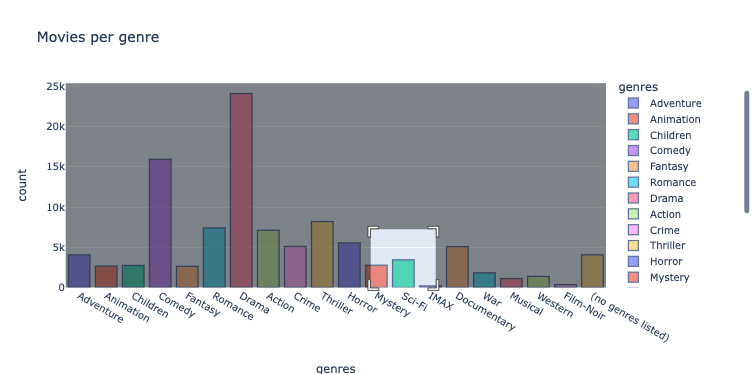
\includegraphics[width=0.4\textwidth]{img/brushing.png}
\caption{\label{fig: LE2 Brushing} Brushing}
\end{figure}

\subsection{Filtering}
Dynamische Abfragen sind eine direkte Möglichkeit, um Daten mit Schiebereglern, Knöpfen und Kategorien zu filtern. 
Sie zeigen globale Eigenschaften auf und helfen bei der Beantwortung spezifischer Fragen ohne Fehlermeldungen. 
Fortgeschrittene Filter erlauben in der Regel OR-Kombinationen innerhalb eines Attributs oder AND-Kombinationen über Attribute hinweg. 
So können komplexere Abfragen gestellt werden.\cite{shneiderman_eyes_1996} \\

\subsection{Implementation mit Dash}

Mit Dash habe ich ein interaktives Dashboard entwickelt, welches die oben genannten Prinzipien implementiert. Das Dashboard ist in Python geschrieben und basiert auf dem Dash Framework. Dash ist ein Framework, welches auf Plotly.js basiert und es ermöglicht interaktive Webanwendungen zu entwickeln.\cite{noauthor_dash_nodate} \\

%add image
\begin{figure}[!h]
\centering
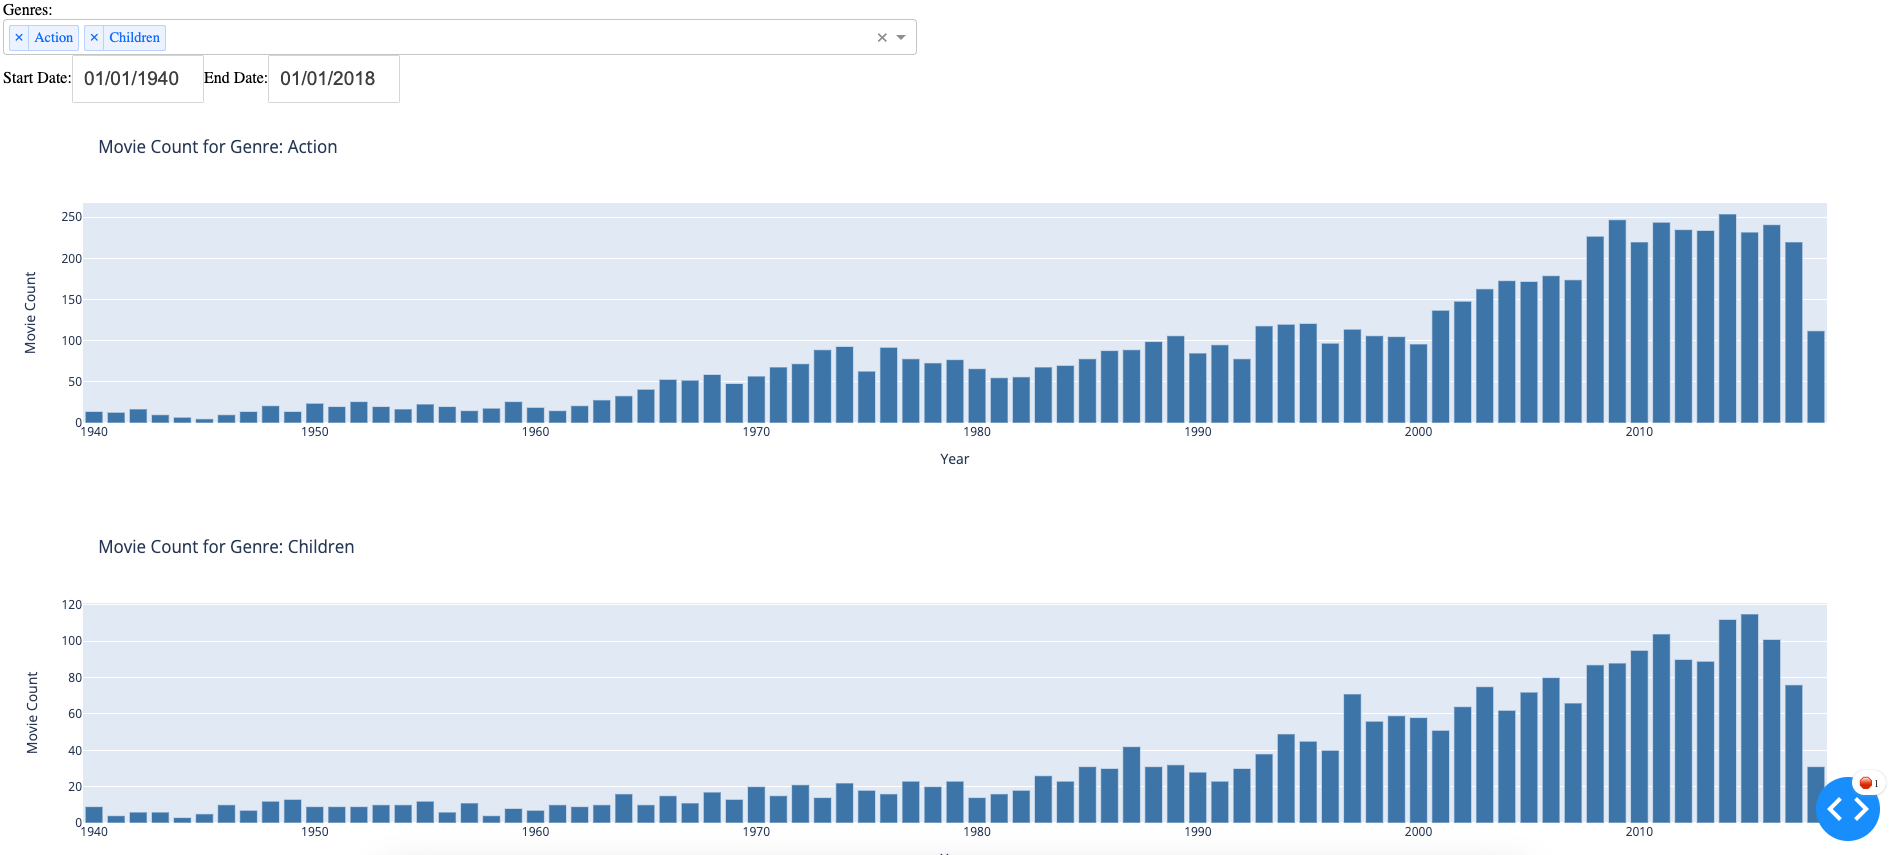
\includegraphics[width=0.4\textwidth]{img/dashboard_plotly.png}
\caption{\label{fig: LE2 Dashboard} Dashboard}
\end{figure}

Mit einem Mulit-Select können die Genres ausgewählt werden. Es wird eine zusätzliche verknüopfte Ansicht angezeigt, welche die Anzahl Filme pro Jahr anzeigt.\\
Zudem kann mit einem Datepicker ein Zeitraum ausgewählt werden. Dieser wird dann in allen anderen Ansichten verwendet.\\

\newpage
\section{LE3: HCI Grundlagen}
Das Ziel von HCI ist es, die Interaktion zwischen Menschen und Computern zu untersuchen und zu verbessern.
In disem Abschnitt werden die Grundlagen von HCI untersucht und die wichtigsten Prinzipien vorgestellt.

\subsection{Fitts's Law}
\noindent
Fitts' Gesetz besagt, dass die Zeit, die benötigt wird, um einen Zeiger zu einem Zielbereich zu bewegen,
 eine Funktion aus Entfernung und Zielgrösse ist. Es wird in der Benutzererfahrung und -schnittstellengestaltung
  verwendet, um Schaltflächen gross zu machen und den Abstand zwischen der Aufgabe und der zugehörigen 
  Schaltfläche kurz zu halten. Es ist wichtig zu beachten, dass dieses Gesetz auf schnelle, 
  zeigende Bewegungen anwendbar ist. Durch die Anwendung dieses Gesetzes haben standardisierte 
  Benutzeroberflächenelemente die Zeit reduziert und die Produktivität gesteigert.\cite{noauthor_what_nodate}
\\
%insert equation here
\begin{equation}
ID = \log_2\left(\frac{2D}{W}\right)
\end{equation}
%erklärung
\begin{center}
ID = Index of Difficulty\\
D = Distance to target\\
W = Width of target\\    
\end{center}

\noindent
Wenn dieses Gesetz auf Figure \ref{fig: LE2 Schneiderman Overview} anwenden. Sollte man mit einer möglichhst kleinen Bewegung die gewünschte Genre auswählen können.
In Plotly kann dies mit dem \texttt{hovermode} umsetzen. So kann zum Beispiel das Genre IMAX sehr schnell ausgewählt werden und muss nicht mit einem präzisen Klick das Genre auswählen.
\begin{figure}[!h]
\centering
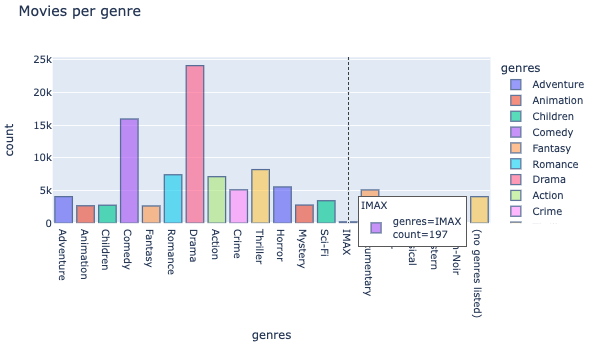
\includegraphics[width=0.4\textwidth]{img/fitts_hover.png}
\caption{\label{fig: LE3 HCI Fitts Law} Fitts's Law hover mode}
\end{figure}

\subsection{Weber's Law}
Webers Gesetz beschreibt die menschliche Fähigkeit,
kleine Unterschiede in Stimuli wie Formen, 
Farben und Gewichten zu erkennen. Es besagt, 
dass das Verhältnis des kleinsten Unterschieds \texttt{$\Delta$I}
den eine Person wahrnehmen kann, zum Anfangsreizwert \texttt{I} für eine bestimmte Messung konstant \texttt{K} ist. 
Die Weber-Fraktion repräsentiert die Steigung dieses Verhältnisses,
 und die Grösse des gerade wahrnehmbaren Unterschieds ist ein konstanter 
 Anteil des ursprünglichen Stimuluswerts. Dieses Gesetz hat Auswirkungen für Grafikdesigner,
  die es nutzen können, um effektivere Benutzeroberflächen zu entwerfen, 
  indem sie sicherstellen, dass es ausreichende Unterscheidung zwischen ähnlichen Stimuli
   wie Linienstärken oder Farbschattierungen gibt.\cite{noauthor_virtual_nodate}

%inset equation here
\begin{equation}
    \frac{\Delta I}{I} = K
\end{equation}

\begin{center}
    $\Delta$I = Delta to Initial Stimulus Value\\
    I = Initial Stimulus Value\\
    K = Weber Fraction\\
\end{center}
\noindent


\newpage

\subsection{5 Dimensionen der Interaktionsgestaltung}
Die fünf Dimensionen der Interaktionsgestaltung wurden von Gillian Crampton Smith, 
Professor am Royal College of Art in London, und Kevin Silver, einem erfahrenen Interaktionsdesigner,
definiert. Die Dimensionen (1D) Worte, (2D) visuelle Darstellungen, 
(3D) physische Objekte/Räume, (4D) Zeit und (5D) Verhalten werden von Interaktionsdesignern genutzt, 
um die Interaktion zwischen Nutzern und einem Produkt oder einer Dienstleistung in ganzheitlicher 
Weise zu betrachten.\cite{noauthor_what_nodate-1}

\noindent
\\
\textbf{1D: Worte}\\
Die Verwendung von passenden und leicht verständlichen Wörtern ist im Interaction Design wichtig, um eine reibungslose Interaktion zwischen dem Benutzer und dem Produkt oder der Dienstleistung zu gewährleisten.
\\
\textbf{2D: Visuelle Darstellungen}\\
Visuelle Elemente wie Bilder, Iconografie und grafische Darstellungen tragen zur Kommunikation zwischen Benutzer und Produkt bei und können genauso wirkungsvoll wie Text sein.
\\
\textbf{3D: Physische Objekte/Räume}\\
Das Medium, über das der Benutzer mit dem Produkt interagiert, wie zum Beispiel ein Mobil- oder Tablet-Bildschirm oder eine Computermaus, muss bei der Gestaltung für eine einfache Benutzerfreundlichkeit berücksichtigt werden.
\\
\textbf{4D: Zeit}\\
Elemente, die sich im Laufe der Zeit verändern, wie Animationen und Videos, können Benutzer einbinden und ihr Erlebnis mit dem Produkt verbessern. Fortschrittsbalken-Animationen können auch hilfreich sein, um den Fortschritt eines bestimmten Prozesses oder einer Operation anzuzeigen.
\\
\textbf{5D: Verhalten}\\
Das tatsächliche Verhalten der Anwendung, einschliesslich Aktionen, Reaktionen und Präsentationen, muss so gestaltet werden, dass es für Benutzer leicht anpassbar und verständlich ist. Zum Beispiel das Anzeigen einer Erfolgsmeldung mit einer Zusammenfassung, wenn eine Aufgabe abgeschlossen 
ist oder das Einbinden von Wischaktionen.\cite{devazya_interaction_2022}

\subsection{Implementation mit Dash}
Rückblickend auf mein Dashboard aus LE2, kann ich sagen, dass ich die meisten dieser Prinzipien umgesetzt habe. Aber es gibt noch einige Punkte, welche ich verbessern könnte.\\
Zum Beispiel bracht es mehr Zeit das Jahr auszuwählen in einem "Date Picker" als in einem Range Slider.\\
Zudem habe ich die verschiedenen Genres mit Hilfe von Farben mehr differenziert und den Hovermode auf der X-Achse aktiviert\\

\begin{figure}[!h]
\centering
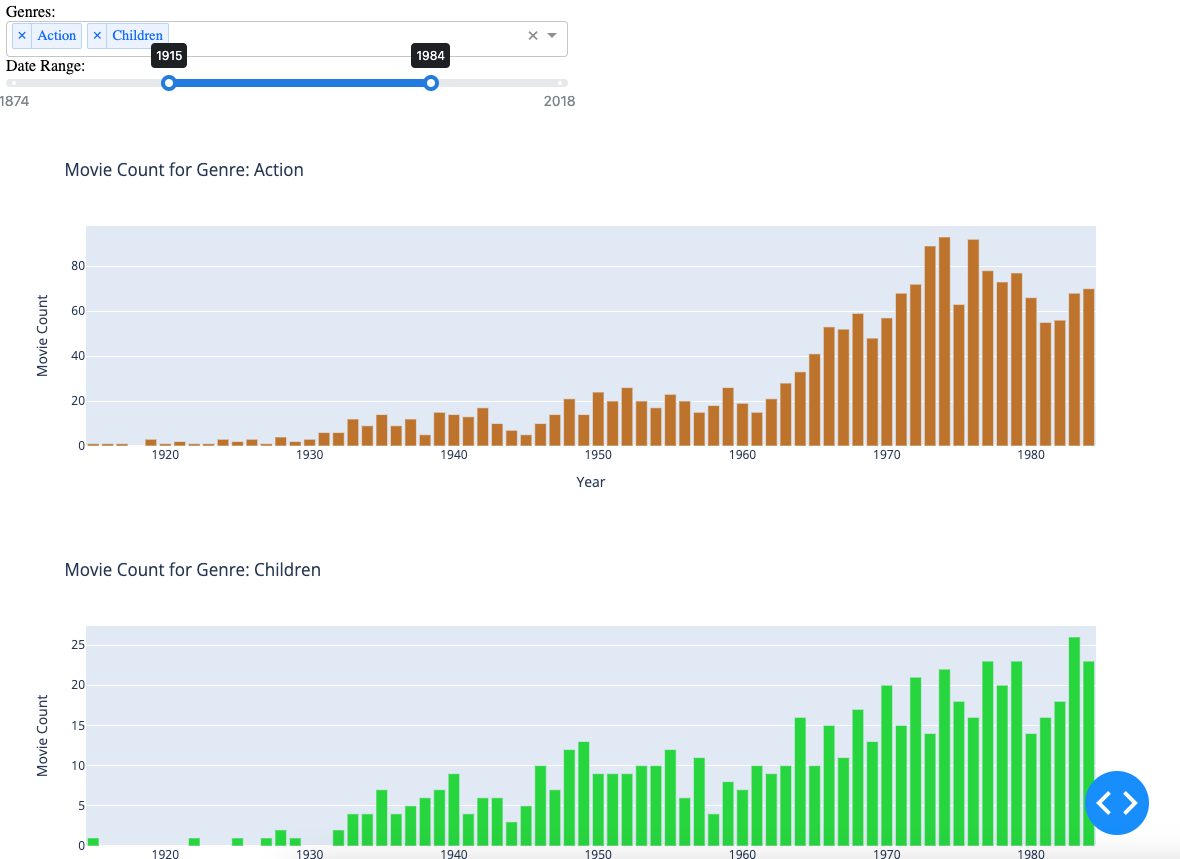
\includegraphics[width=0.3\textwidth]{img/dashboard_updated.png}
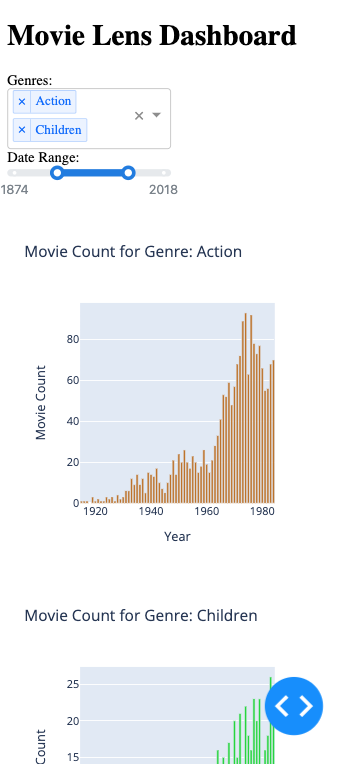
\includegraphics[height=0.25\textwidth]{img/dashboard_mobile.png}
\caption{\label{fig: LE3 Dashboard mit Verbesserungen / Mobile} Dashboard mit Verbesserungen / Mobile}
\end{figure}
\noindent
Zudem habe ich die dritte Dimension der Interaktionsgestaltung untersucht. Wie sieht das Dashboard auf einem Smartphone aus?\\
Können die verschiedenen Elemente noch gut ausgewählt werden?\\
Kann man die Daten gleich gut interpretieren?\\

\newpage
\section{LE4: Evaluierung}

Im Rahmen von LE4 werde ich ein kleine Nutzerstudie zu meinem erstellten Dashboard durchführen, um die Usability und User Experience zu evaluieren. 
Dabei werde ich die im Kurs "GDV" erworbenen Kenntnisse nutzen.

\subsection{Usability Test}
Der Usability Test ist eine Methode, um die Benutzerfreundlichkeit eines Produkts zu bewerten, indem es von echten Benutzern getestet wird.
Das Test Set-Up ist wie folgt: Es werden 3 Testpersonen ausgewählt, welche das Dashboard testen sollen.
Die Testpersonen werden gebeten, die Aufgaben zu lösen und dabei wird die Zeit gemessen und ob ihre Antwort korrekt ist\\

\noindent
Die Personen sind mit der Benutzung von Computer vertraut, haben aber keine signifikanten Erfahrungen mit Dashboards.
Alle Personen sind im Alter von 20-30 Jahren und verstehen Englisch.\\
\\
Aufgaben:
\begin{enumerate}
    \item Wähle das Genre IMAX vom Jahr 1950 bis 2015.
    \item Vergleiche Genre Action und Adventure. Welches Genre hat mehr Filme im Jahr 1975?
    \item Wahr oder Falsch? Es gibt mehr Filme im Genre Action als im Genre Adventure von 1975 bis 200.
    \item Welches Genre hat am meisten Filme von 2000 bis 2015?
    \item Welches Genres hat am meisten Filme über die ganze Zeit?
\end{enumerate}

Correct Answers will be marked with a \texttt{+} and wrong answers with a \texttt{-}.\\

\begin{equation}
    Precission = \frac{Correct Answers}{Total Answers}\\
\end{equation}


\subsubsection{Ergebnisse}
Zeitformat: MM:SS\\
\begin{table}[!h]
    \centering
    \begin{tabular}{|l|l|l|l|l|}
    \hline
    \textbf{Aufgabe} & \textbf{Testperson 1} & \textbf{Testperson 2} & \textbf{Testperson 3} & \textbf{Durchschnitt}\\
    \hline
    1 & 00:23 + & 00:25 + & 00:21 + & 00:23\\
    \hline
    2 & 00:27 + & 00:29 + & 00:25 + & 00:27\\
    \hline
    3 & 00:42 + & 00:57 -& 00:38 + & 00:46\\
    \hline
    4 & nAn -& nAn -& nAn -& nAn\\
    \hline
    5 &nAn -& nAn -& nAn -& nAn\\
    \hline
    Total & 01:32 (60\%) & 01:51 (40\%)& 01:24 (60\%) & 01:36\\
    \hline
    \end{tabular}
    \caption{\label{tab: LE4 Usability Test}Usability Test Ergebnisse}
\end{table}

\noindent
Zu beobachten waren sehr gute Ergebnisse für Aufgabe 1 und 2. Bei Aufgabe 3 und 4 benötigen die Testpersonen etwas länger und waren mit ihren Antworten nicht immer korrekt.
Bei Aufgabe 5 hatten alle Testpersonen lange und konnten die Aufgabe nicht lösen.\\
\noindent
Wichtigste Erkentnisse aus qualitativem Feedback:
\begin{itemize}
    \item Die Bar Plot sollten kombiniert werden. Die Testpersonen mussten mit Scrollen die Genres vergleichen.
    \item Es fehlt eine Übersicht pro Genres die totale Anzahl für den ausgewählten Zeitraum darstellt.
    \item Wenn man alle Genres auswählen möchte dauert es sehr lange. Es sollte eine Möglichkeit geben alle Genres auszuwählen.
\end{itemize}
\newpage

\subsection{Dashboard Redesign}

Die oben genannte Punkte wurden in einem Redesign des Dashboards umgesetzt.\\
Die Bar Plots wurden kombiniert und ein Total vom ausgewählten Zeitraum wurde hinzugefügt.\\
Zudem wurde ein Preset hinzugefügt, welches alle Genres auswählt.\\

\begin{figure}[!h]
\centering
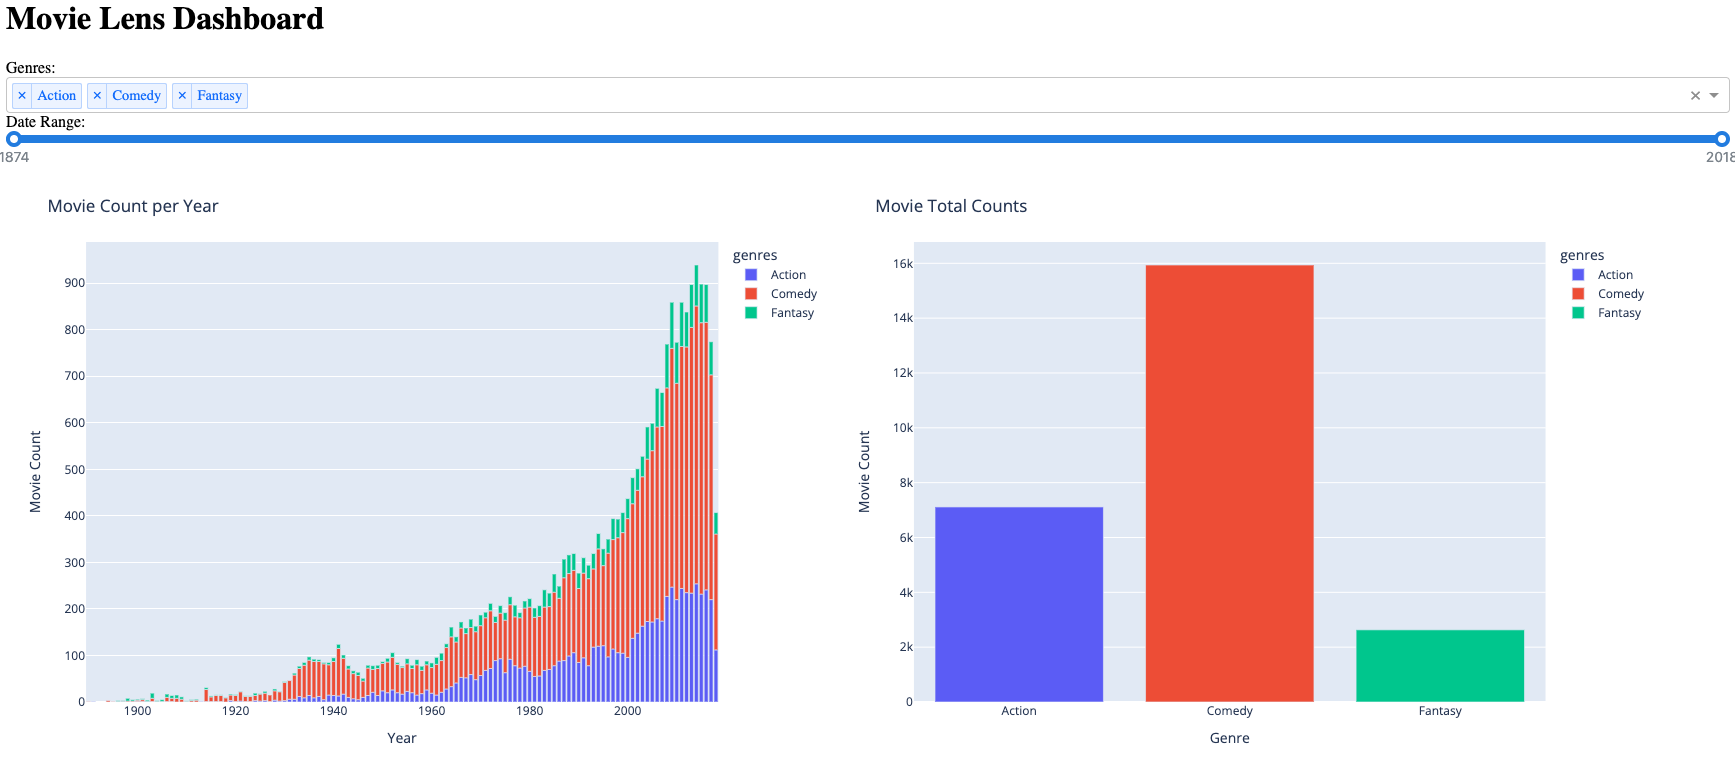
\includegraphics[width=0.4\textwidth]{img/dashboard_redesign.png}
\caption{\label{fig: LE4 Dashboard Redesign} Dashboard Redesign}
\end{figure}

\subsubsection{Usability Test nach Redesign}
Mit den selben Testpersonen wurde ein Usability Test nach dem Redesign durchgeführt.\\
Zu erwähnen ist, dass die Testpersonen bereits mit dem Dashboard vertraut waren und somit einen Lerneffekt hatten.\\
Das heisst sie kennen bereits die Grundmechanismen und können das Dashboard schneller bedienen.\\



\subsubsection{Ergebnisse nach Redesign}
Zeitformat: MM:SS\\
\begin{table}[!h]
    \centering
    \begin{tabular}{|l|l|l|l|l|l|}
    \hline
    \textbf{Aufgabe} & \textbf{Testperson 1} & \textbf{Testperson 2} & \textbf{Testperson 3} & \textbf{Durchschnitt} & \textbf{Delta nach Redesign}\\
    \hline
    1 & 00:16 + & 00:19 + & 00:21 + & 00:19 & -00:04\\
    \hline
    2 & 00:09 + & 00:15 + & 00:08 + & 00:11 & -00:16\\
    \hline
    3 & 00:34 + & 00:37 +& 00:31 + & 00:34 & -00:12\\
    \hline
    4 & 00:18 +& 00:24 +& 00:15 +& 00:19 & nAn\\
    \hline
    5 &00:06 +& 00:10 +& 00:05 +& 00:07 & nAn\\
    \hline
    Total & 01:23 (100\%) & 01:45 (100\%)& 01:20 (100\%)& 01:30 & -00:06\\
    \hline
    \end{tabular}
    \caption{\label{tab: LE4 Usability Test}Usability Test Ergebnisse}
\end{table}
Zu beobachten ist eine signifikante Verbesserung der Zeit für die Aufgaben 1-3.\\
Die Aufgaben 4 und 5 konnten nun gelöst werden. Aber die Zeit kann nicht verglichen werden, da die Aufgaben vorher nicht gelöst werden konnten.\\
Die Gesamtzeit konnte um 6 Sekunden verbessert werden. Jedoch ist auch diese Zeit schwiriger zu interpretieren, da 2 von 5 Aufgaben nicht gelöst werden konnten im ersten Durchlauf.\\
Gesamthaft konnte die Precission von 53\% auf 100\% verbessert werden.\\
\\
Bei den qualitativen Feedbacks wurde erwähnt, dass die Testpersonen das Redesign besser finden.\\
Auch die Option alle Genres auszuwählen wurde positiv aufgenommen.\\
Der zusätzliche Total Wert wurde als sehr hilfreich empfunden wenn man Zahlen über die Zeit vergleichen möchte.\\
Das Kombinieren der Genres Graphen wurde auch als angenehm empfunden. Da mann weniger scrollen muss um die Daten zu vergleichen.\\

\newpage
\printbibliography

\newpage

\section{Anhang}
% add all figures again here in full size
\centering
\subsection{Figure 1}
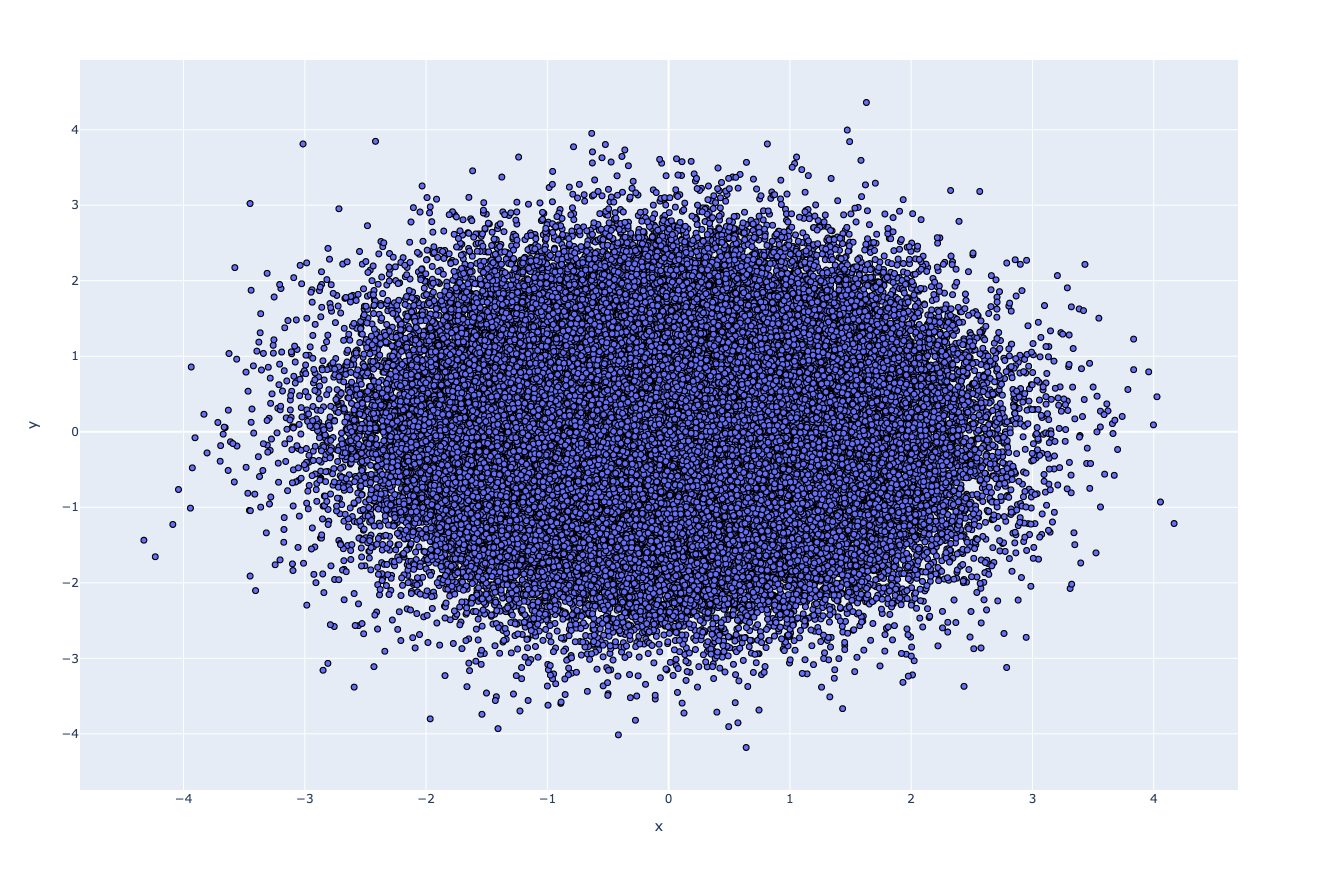
\includegraphics[width=1\textwidth]{img/random_dots.png}

\subsection{Figure 2}
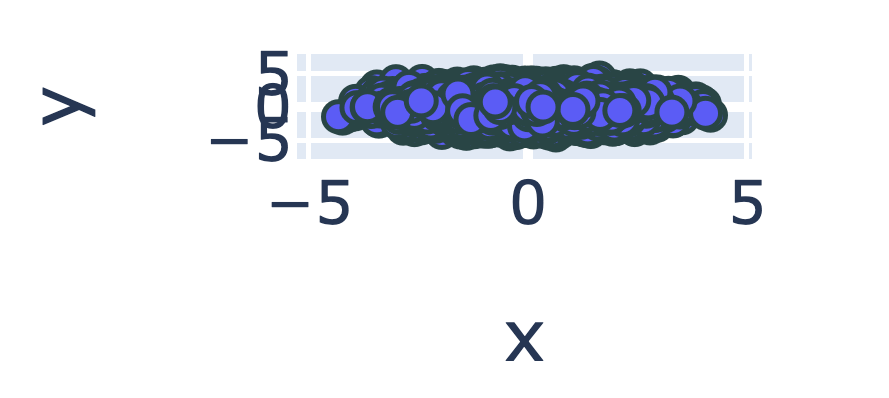
\includegraphics[width=0.7\textwidth]{img/svg_quality.png}
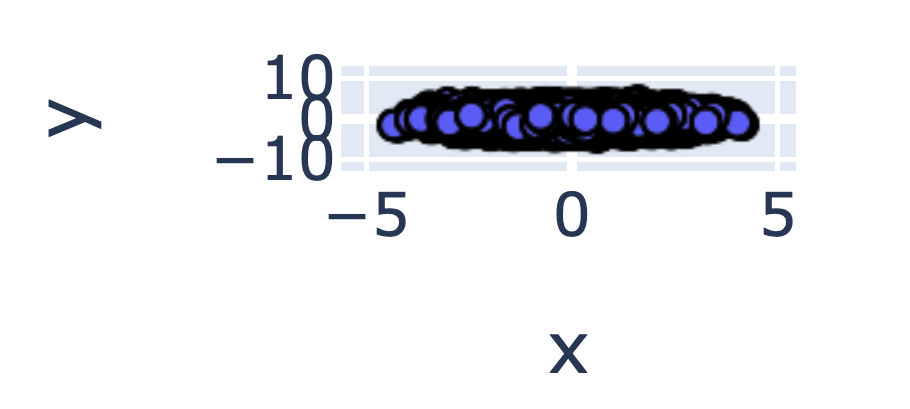
\includegraphics[width=0.7\textwidth]{img/webgl_quality.png}

\subsection{Figure 3}
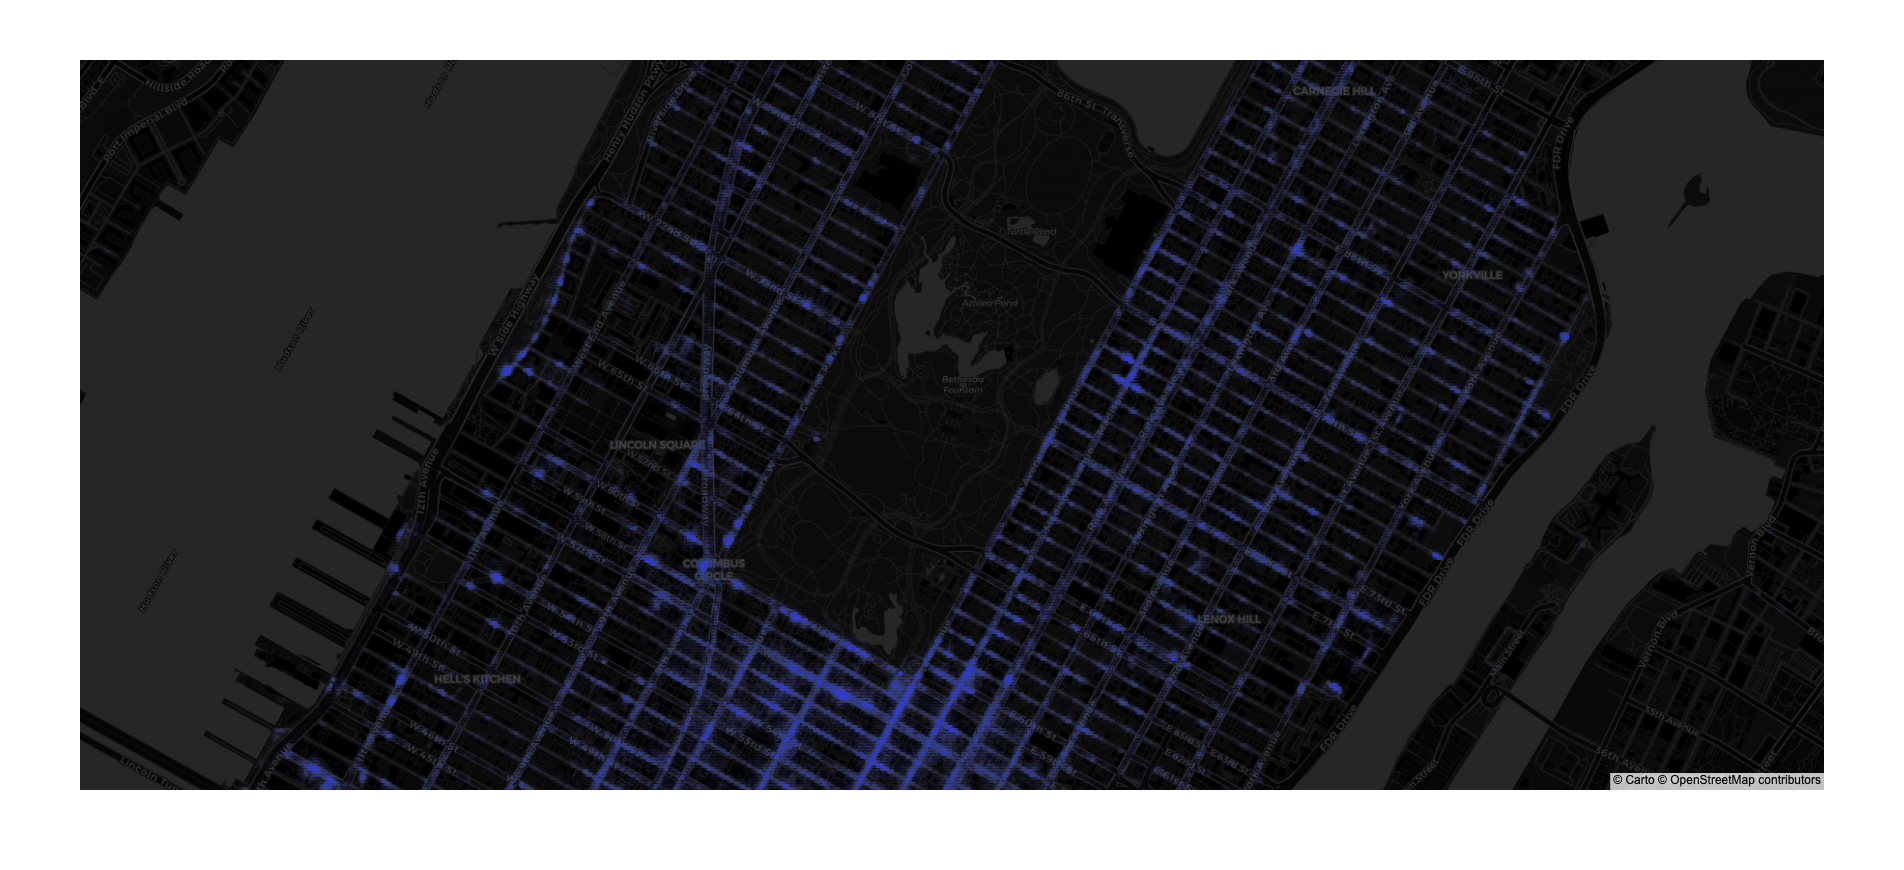
\includegraphics[width=1\textwidth]{img/newyork_plotly.png}
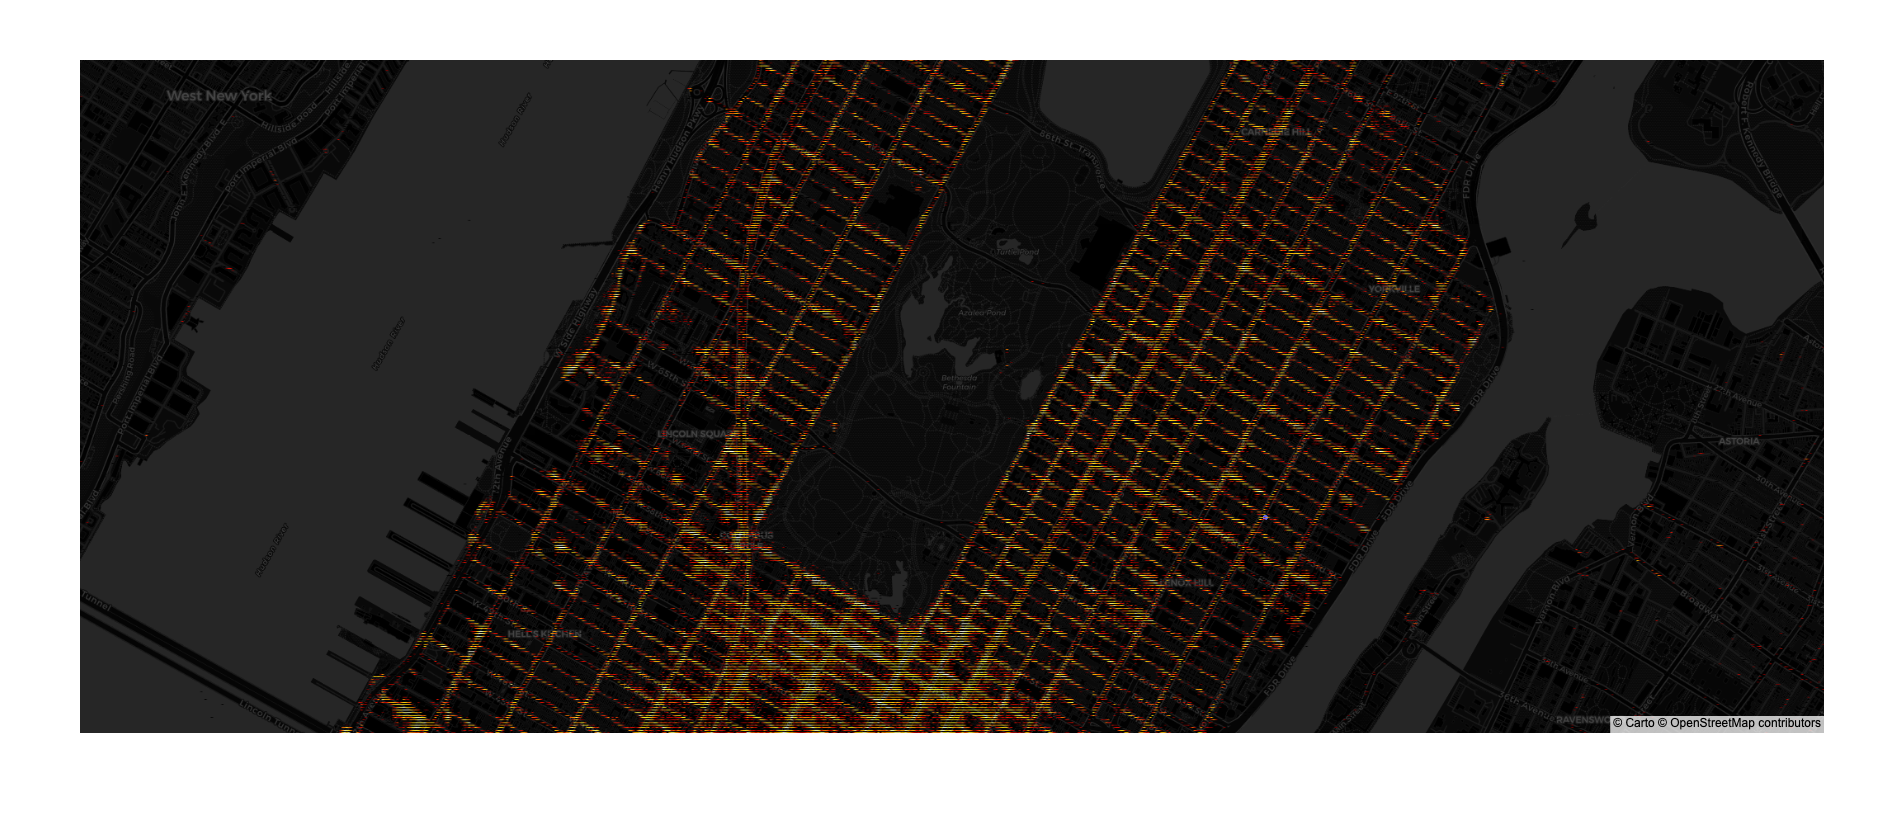
\includegraphics[width=1\textwidth]{img/newyork_datashader.png}

\subsection{Figure 4}
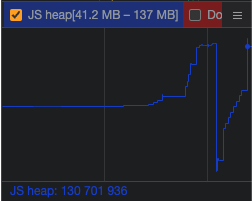
\includegraphics[width=0.6\textwidth]{img/js_heap_plotly.png}
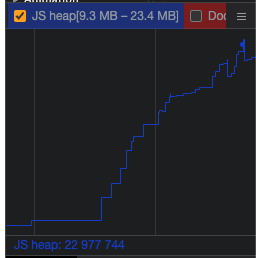
\includegraphics[width=0.6\textwidth]{img/js_heap_datashader.png}

\subsection{Figure 5}
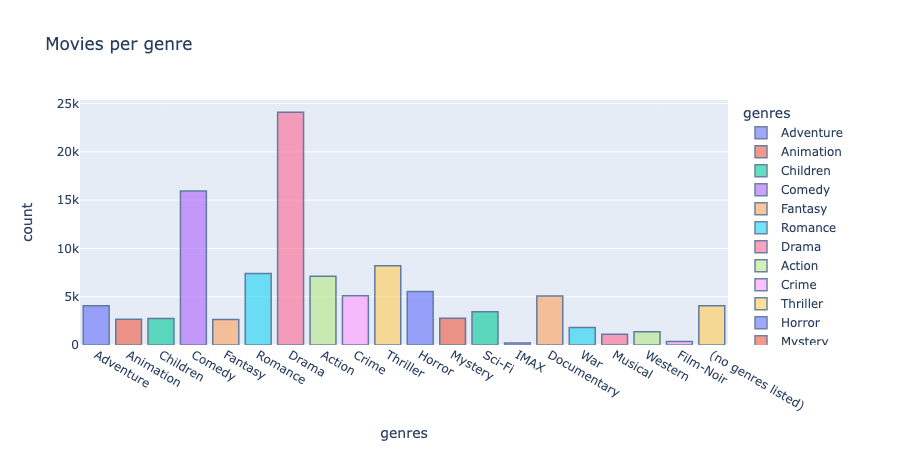
\includegraphics[width=1\textwidth]{img/movies_genre.png}

\subsection{Figure 6}
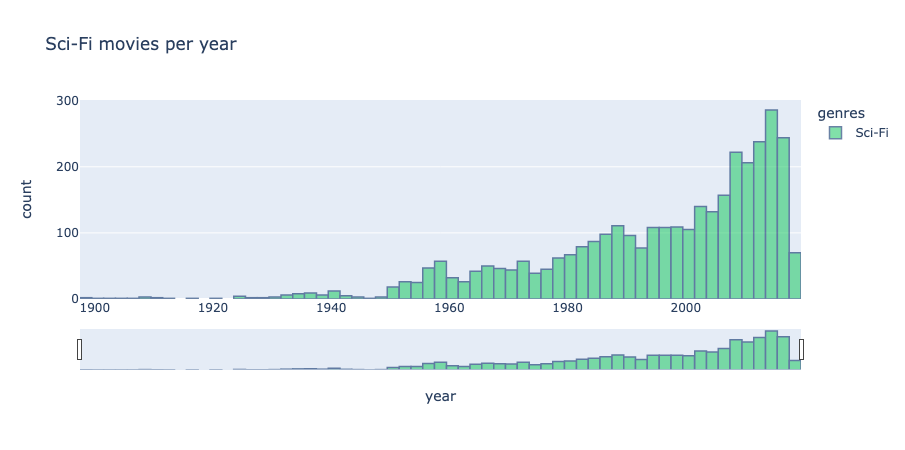
\includegraphics[width=1\textwidth]{img/movies-scifi.png}

\subsection{Figure 7}
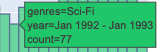
\includegraphics[width=0.4\textwidth]{img/tooltip.png}

\subsection{Figure 8}
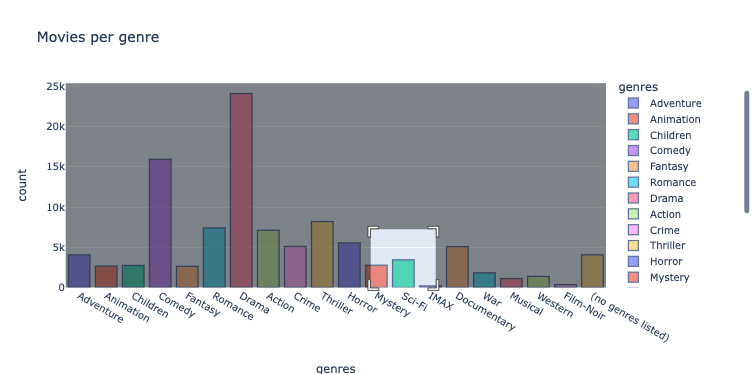
\includegraphics[width=1\textwidth]{img/brushing.png}

\subsection{Figure 9}
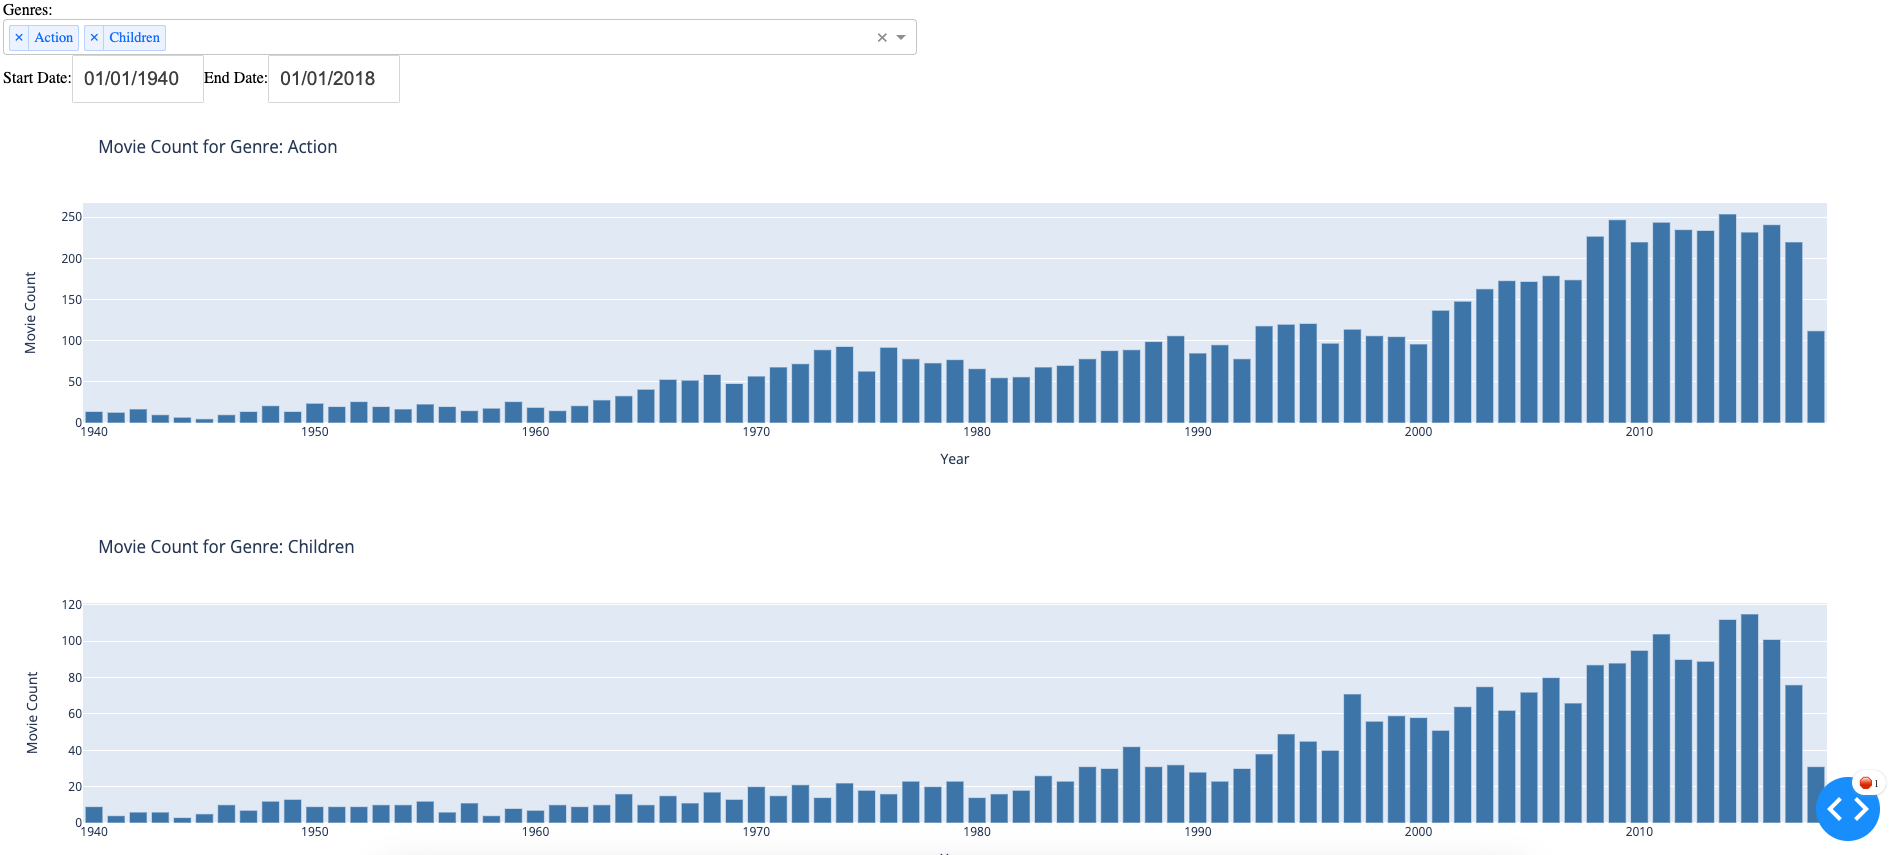
\includegraphics[width=1\textwidth]{img/dashboard_plotly.png}

\subsection{Figure 10}
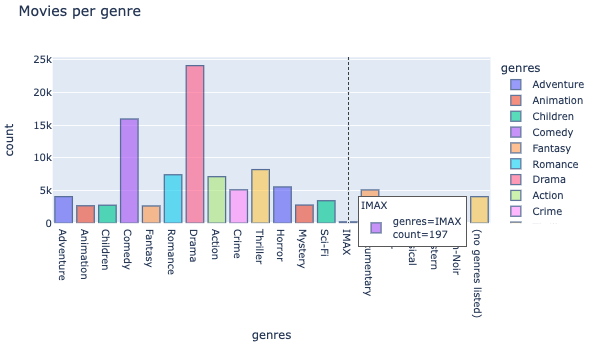
\includegraphics[width=1\textwidth]{img/fitts_hover.png}

\subsection{Figure 11}
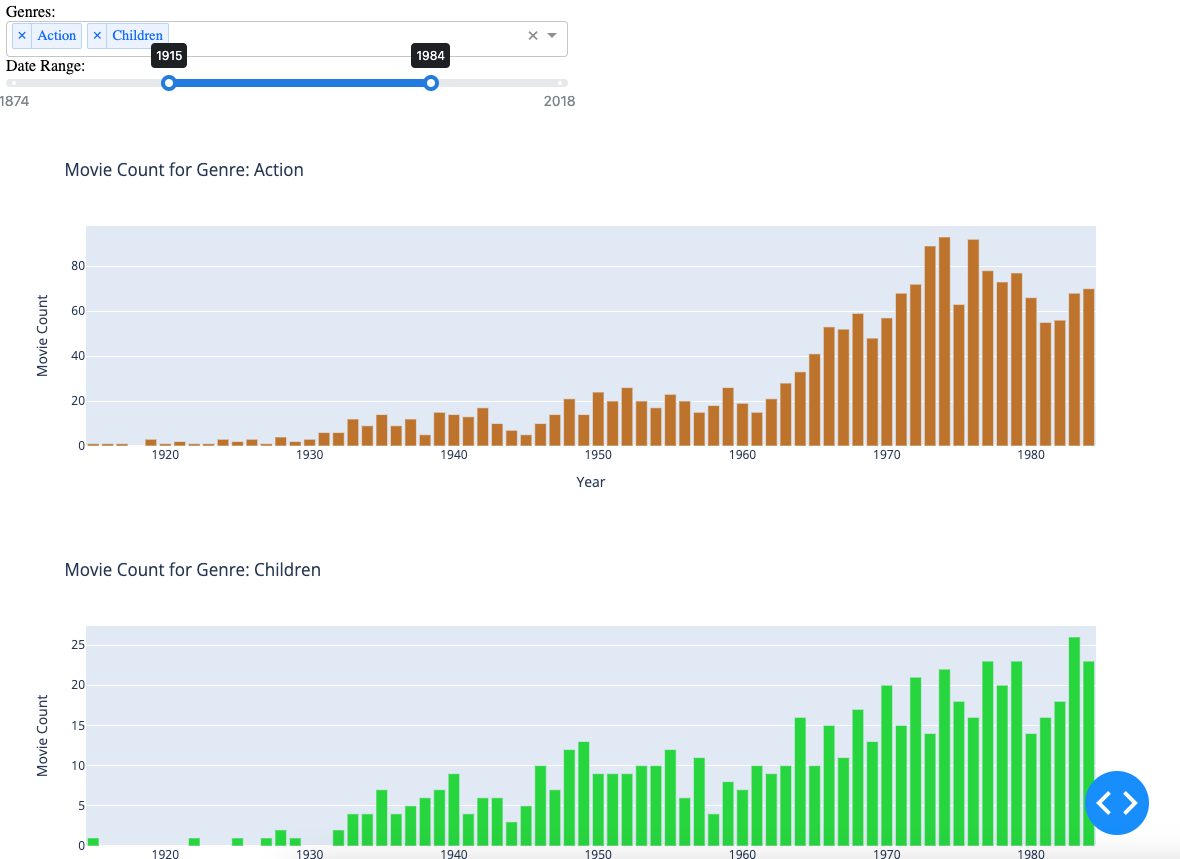
\includegraphics[width=1\textwidth]{img/dashboard_updated.png}\\
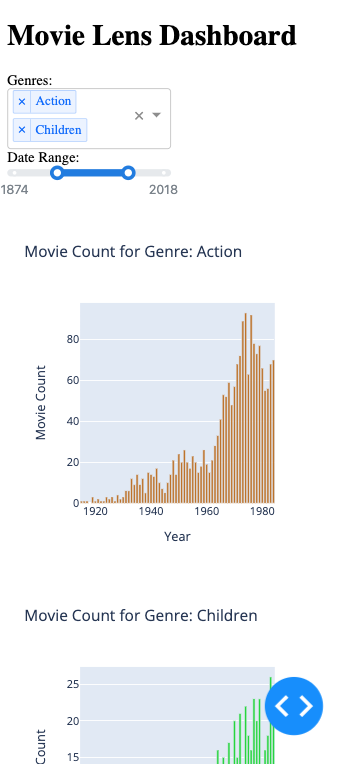
\includegraphics[width=0.4\textwidth]{img/dashboard_mobile.png}

\subsection{Figure 12}
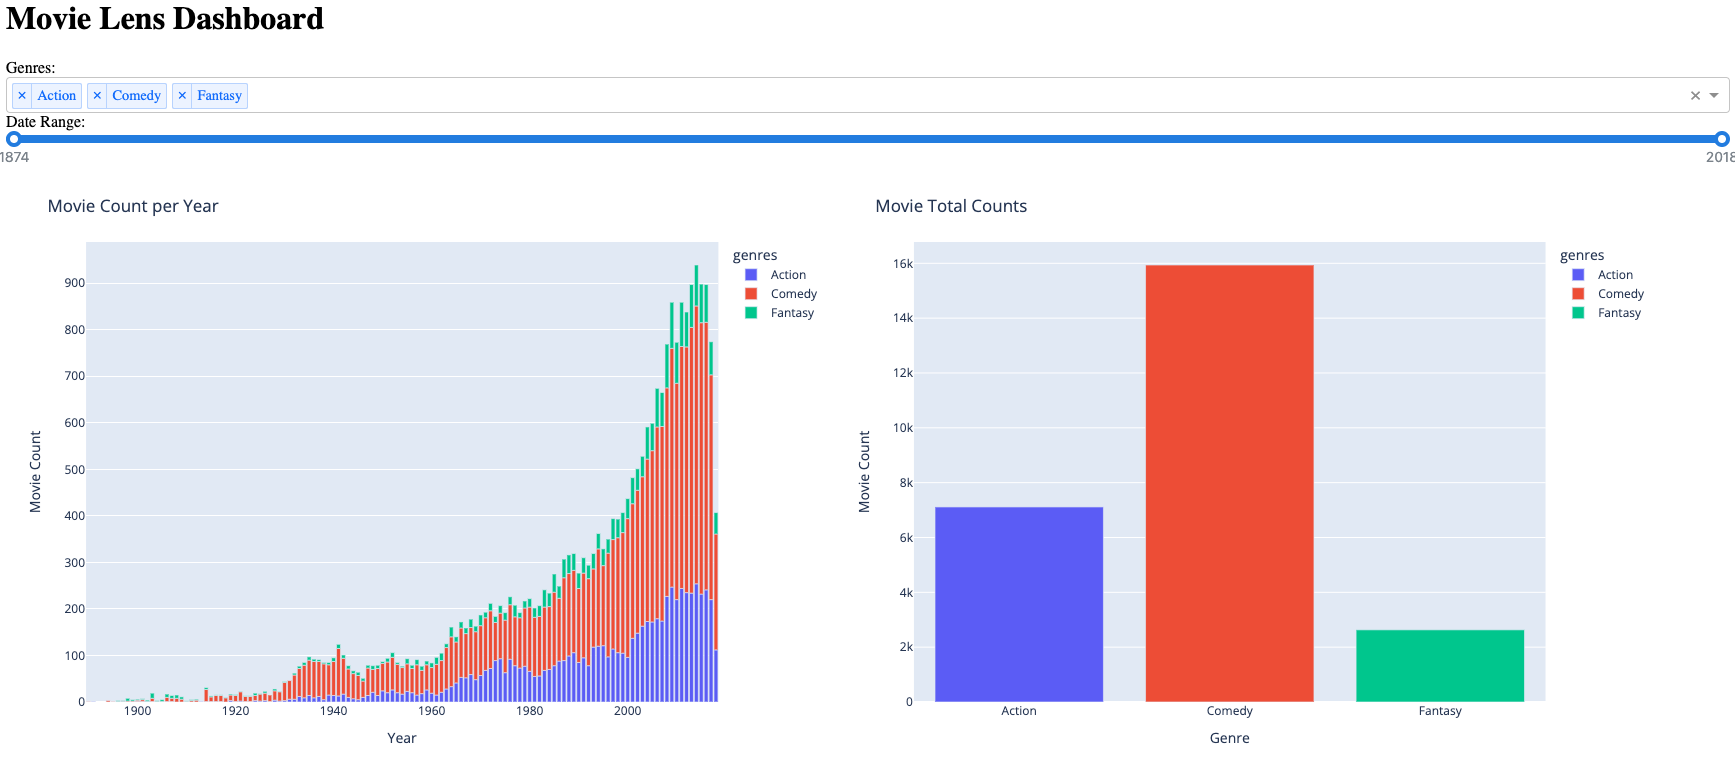
\includegraphics[width=1\textwidth]{img/dashboard_redesign.png}
  
\end{document}